\documentclass[a5paper, 10pt]{article}

% Текст
\usepackage[utf8]{inputenc} % UTF-8 кодировка
\usepackage[russian]{babel} % Русский язык
\usepackage{indentfirst} % красная строка в первом параграфе в главе
% Отображение страниц
\usepackage{geometry} % размеры листа и отступов
\geometry{
	left=12mm,
	top=25mm,
	right=15mm,
	bottom=17mm,
	marginparsep=0mm,
	marginparwidth=0mm,
	headheight=10mm,
	headsep=7mm,
	nofoot}
\usepackage{afterpage,fancyhdr} % настройка колонтитулов
\pagestyle{fancy}
\fancypagestyle{style}{ % создание нового стиля style
	\fancyhf{} % очистка колонтитулов
	\fancyhead[LO, RE]{} % название документа наверху
	\fancyhead[RO, LE]{\leftmark} % название section наверху
	\fancyfoot[RO, LE]{\thepage} % номер страницы справа внизу на нечетных и слева внизу на четных
	\renewcommand{\headrulewidth}{0.25pt} % толщина линии сверху
	\renewcommand{\footrulewidth}{0pt} % толцина линии снизу
}
\fancypagestyle{plain}{ % создание нового стиля plain -- полностью пустого
	\fancyhf{}
	\renewcommand{\headrulewidth}{0pt}
}
\fancypagestyle{title}{ % создание нового стиля title -- для титульной страницы
	\fancyhf{}
	\fancyhead[C]{{\footnotesize
			Министерство образования и науки Российской Федерации\\
			Федеральное государственное автономное образовательное учреждение высшего образования
	}}
	\fancyfoot[C]{{\large 
			Санкт-Петербург, 2023
	}}
	\renewcommand{\headrulewidth}{0pt}
}

% Математика
\usepackage{amsmath, amsfonts, amssymb, amsthm} % Набор пакетов для математических текстов
%\usepackage{dmvnbase} % мехматовский пакет latex-сокращений
\usepackage{cancel} % зачеркивание для сокращений
% Рисунки и фигуры
\usepackage[pdftex]{graphicx} % вставка рисунков
\usepackage{wrapfig, subcaption} % вставка фигур, обтекая текст
\usepackage{caption} % для настройки подписей
\captionsetup{figurewithin=none,labelsep=period, font={small,it}} % настройка подписей к рисункам
% Рисование
\usepackage{tikz} % рисование
\usepackage{circuitikz}
\usepackage{pgfplots} % графики
% Таблицы
\usepackage{multirow} % объединение строк
\usepackage{multicol} % объединение столбцов
% Остальное
\usepackage[unicode, pdftex]{hyperref} % гиперссылки
\usepackage{enumitem} % нормальное оформление списков
\setlist{itemsep=0.15cm,topsep=0.15cm,parsep=1pt} % настройки списков
% Теоремы, леммы, определения...
\theoremstyle{definition}
\newtheorem{Def}{Определение}
\newtheorem*{Axiom}{Аксиома}
\theoremstyle{plain}
\newtheorem{Th}{Теорема}
\newtheorem{Lem}{Лемма}
\newtheorem{Cor}{Следствие}
\newtheorem{Ex}{Пример}
\theoremstyle{remark}
\newtheorem*{Note}{Замечание}
\newtheorem*{Solution}{Решение}
\newtheorem*{Proof}{Доказательство}
% Свои команды
\newcommand{\comb}[1]{\left[\hspace{-4pt}\begin{array}{l}#1\end{array}\right.\hspace{-5pt} } % совокупность уравнений
% Титульный лист
\usepackage{csvsimple-l3}
\newcommand*{\titlePage}{
	\thispagestyle{title}
	\begingroup
	\begin{center}
		%		{\footnotesize
			%			Министерство образования и науки Российской Федерации\\
			%			Федеральное государственное автономное образовательное учреждение высшего образования
			%		}
		%		
		\vspace*{6ex}
		
		{\small
			САНКТ-ПЕТЕРБУРГСКИЙ НАЦИОНАЛЬНЫЙ ИССЛЕДОВАТЕЛЬСКИЙ УНИВЕРСИТЕТ ИТМО
		}
		
		\vspace*{2ex}
		
		{\normalsize
			Факультет систем управления и робототехники
		}
		
		\vspace*{15ex}
		
		{\Large \bfseries 
			Лабораторная работа  №5
		}

                     \vspace*{2ex}
{\Large \bfseries 
			"Стабилизация перевернутого маятника"
		}

                     \vspace*{2ex}
		
		{\normalsize
			по дисциплине "Введение в профессиональную деятельность. Проектная деятельность."
		}
                     \vspace*{2ex}
	\end{center}
	\vspace*{10ex}
	\begin{flushright}
		{\large 
			\underline{Выполнили}: студенты гр. \textbf{R3138}\\
			\begin{flushright}
				\textbf{Иванов А. К.}\\
                                           \textbf{Нечаева А. А.}\\
                                           \textbf{Велюго К. О.}\\
                                           \textbf{Воротников А. А.}\\
			\end{flushright}
		}
		
		\vspace*{5ex}
		
		{\large 
			\underline{Преподаватель}: \textit{Перегудин А.А.}
		}
	\end{flushright}	
	\newpage
	\setcounter{page}{2}
	\endgroup}

\begin{document}
	\titlePage
	\pagestyle{style}


\newpage
\section{Цель работы}
Стабилизация перевернутого маятника с помощью выведенного закона управления.
\section{Теоретическая часть}	
В данной работе все построения выполняются для простой модели перевернутого маятника на тележке, движение которого осуществляется в плоскости.

\subsection{Вывод формул и построение математической модели}	
Основные величины, необходимые для построения математической модели перевернутого маятника (Рисунок 1):\\
$\Theta $ -- угловое отклонение маятника от положения равновесия;\\
$l$ -- длина маятника;\\
$m_1$ -- масса груза (считаем, что вся масса маятника сосредоточена на его конце);\\
$m_2$ -- масса тележки, на которой закреплен маятник;\\
$F$ -- сила, действующая на тележку.\\
Второй закон Ньютона в случае вращательного движения запишется:
\begin{equation}
\ddot{\Theta}I = M \, ,
\end{equation}
где $\ddot{\Theta}$ -- угловое ускорение маятника, $I$ -- момент инерции маятника, $M$ -- момент вращающей силы.\\
Момент инерции для стержня, вращающегося вокруг одного из концов:
\begin{equation}
I = m_1 \cdot l^2 \, ,
\end{equation}
$m_1$ -- масса груза, $l$ -- длина стержня.\\
Вращающая сила, действующая на маятник -- сила тяжести, поэтому момент силы перепишется в следующем виде:
\begin{equation}
M = m_1 g l \sin \Theta \, 
\end{equation}
Далее подставляем выражения для момента инерции (2) и момента силы (3) в уравнение (1):
 
\begin{equation}
\ddot{\Theta}  m_1 \cdot l^2  = m_1 g l  \sin \Theta \to \ddot{\Theta} = \frac{g}{l} \sin \Theta
\end{equation}
Далее запишем кинетическую энергию системы "тележка-маятник":
\begin{equation}
E_{sum} = E_{pen} + E_{cart} = \frac{m_1 v_1^2}{2} +  \frac{(m_2 + m_1) v_2^2}{2} \, ,
\end{equation}
где $ E_{pen}$ -- кинетическая энергия маятника, $ E_{cart}$ -- кинетическая энергия тележки, $v_1$ -- скорость груза, $v_2$ -- скорость тележки.\\
Запишем выражения для соотвествующих скоростей:\\
 скорость тележки -- изменение ее координаты по времени
\begin{equation}
v_2 = \frac{dx}{dt} = \dot{x} \, ;
\end{equation}
скорость груза -- измение его координат по времени:
\begin{multline}
v_1 = \sqrt{\left( \frac{d \left( x + l \sin \Theta  \right)}{dt} \right)^2 + \left(  \frac{d l \cos \Theta }{dt}  \right)^2} = \\
= \sqrt{\left( \dot{x} + \dot{\Theta} l \cos \Theta \right)^2 + \left( -  \dot{\Theta} l \sin \Theta \right)^2} = 
 \sqrt{\dot{x}^2 +2 \dot{x} \dot{\Theta} l \cos \Theta +  \dot{\Theta}^2 l^2}
\end{multline}
В итоге получаем выражение для полной кинетической энергии системы:
\begin{equation}
E_{sum} = E_{pen} + E_{cart} = \frac{m_1 (\dot{x}^2 +2 \dot{x} \dot{\Theta} l \cos \Theta +  \dot{\Theta}^2 l^2)}{2} +  \frac{(m_2 + m_1) \dot{x}^2}{2} 
\end{equation}
Далее выразим силу, действующую на систему:
\begin{equation}
F = (m_1 + m_2) \ddot{x} + m_1 l \ddot{\Theta} \cos \Theta - m_1 l \dot{\Theta} ^2 \sin \Theta
\end{equation}
И, воспользовавшись уравнениями Лагранжа, получим систему:
\begin{equation}
\begin{cases}
F = (m_1 + m_2) \ddot{x} + m_1 l \ddot{\Theta} \cos \Theta - m_1 l \dot{\Theta} ^2 \sin \Theta \, , \\
l \ddot{\Theta} + g \sin \Theta = \ddot{x} \cos \Theta
\end{cases}
\end{equation} 
Проведем математические преобразования:
\begin{equation}
l \ddot{\Theta} + g \sin \Theta = \ddot{x} \cos \Theta \to  \ddot{x} = \frac{l \ddot{\Theta} + g \sin \Theta }{ \cos \Theta}
\end{equation}
\begin{equation}
F = (m_1 + m_2) \frac{l \ddot{\Theta} + g \sin \Theta }{ \cos \Theta} + m_1 l \ddot{\Theta} \cos \Theta - m_1 l \dot{\Theta} ^2 \sin \Theta \,
\end{equation}
Выразим угловое ускорение:
\begin{equation}
\ddot{\Theta} = \frac{\left( F - \frac{(m_1 + m_2) g \sin \Theta}{\cos \Theta} + m_1 l \dot{\Theta}^2 \sin \Theta \right) \cos \Theta}{l \left( m_1 + m_2 + m_1 \cos^2 \Theta \right)}
\end{equation}

\newpage
\section{Практическая часть}	
\subsection{Управляющий закон}
Для стабилизации маятника использовался ПИД-регулятор.
\subsection{Построение схемы в Simulink}
\begin{figure}[h]
		\center{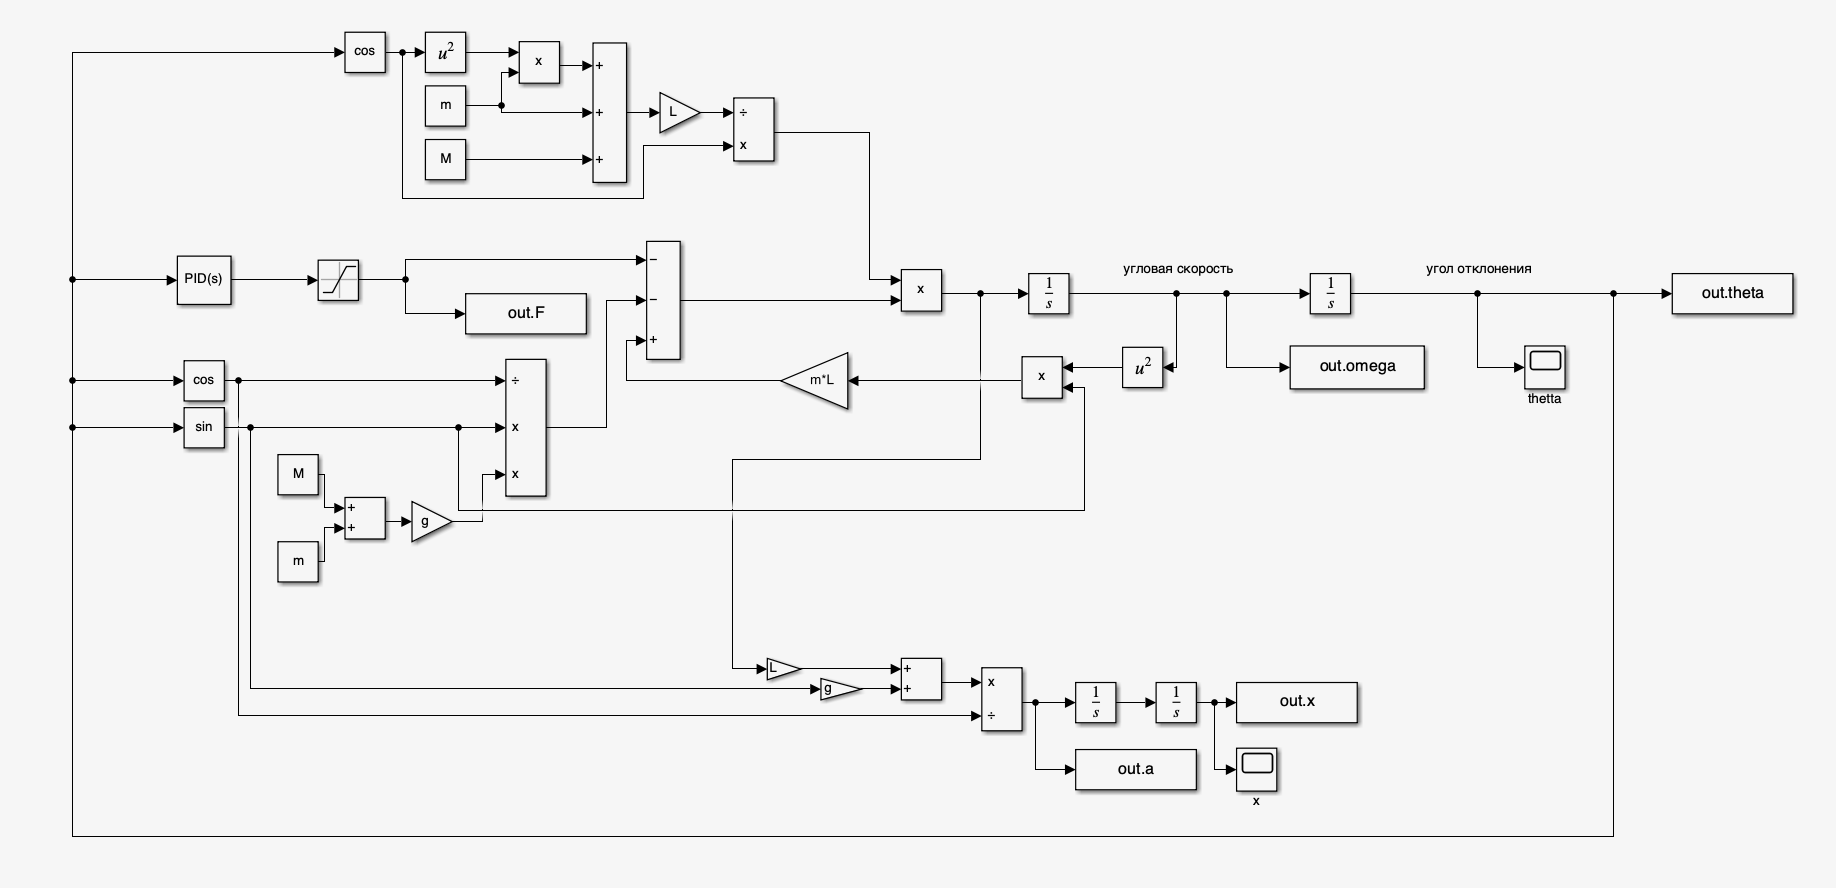
\includegraphics[width=1\linewidth]{"./graphics/sim.png"}}
                    %  \includegraphics{"./Q-table.jpg"}
	           \caption{Схема}
\end{figure}
Для моделирования процесса стабилизации маятника использовалась схема, приведенная на рисунке 1.
\subsection{Результаты}
В результате были получены графики (рисунки 2 - 9) зависимости угла отклонения маятника от вертикали ($\Theta (t)$) и координаты центра тележки ($x(t)$) для различных наборов коэффициентов ПИД-регулятора.

\subsection{Вывод}
В процессе выполнения лабораторной работы была выведена математическая модель перевернутого маятника на основе уравнений механики, синтезирован закон управления и проведен подбор параметров для стабилизации маятника. Наиболее оптимальными коэффициентами для стабилизации маятника в данной работе были выбраны  $p = 20, \, i = 10, \, d = 0$ (Рисунок 6), где $p$ -- коэффиент пропорциональности, $i$ -- коэффициент перед интегральной составляющей, $d$ -- перед дифференциальной составляющей. Об успешной стабилизации говорит отсутствие видимой на графике установившейся ошибки, относительно небольшое перерегулирование и короткое время стабилизации процесса.

\begin{figure}[!h]
		{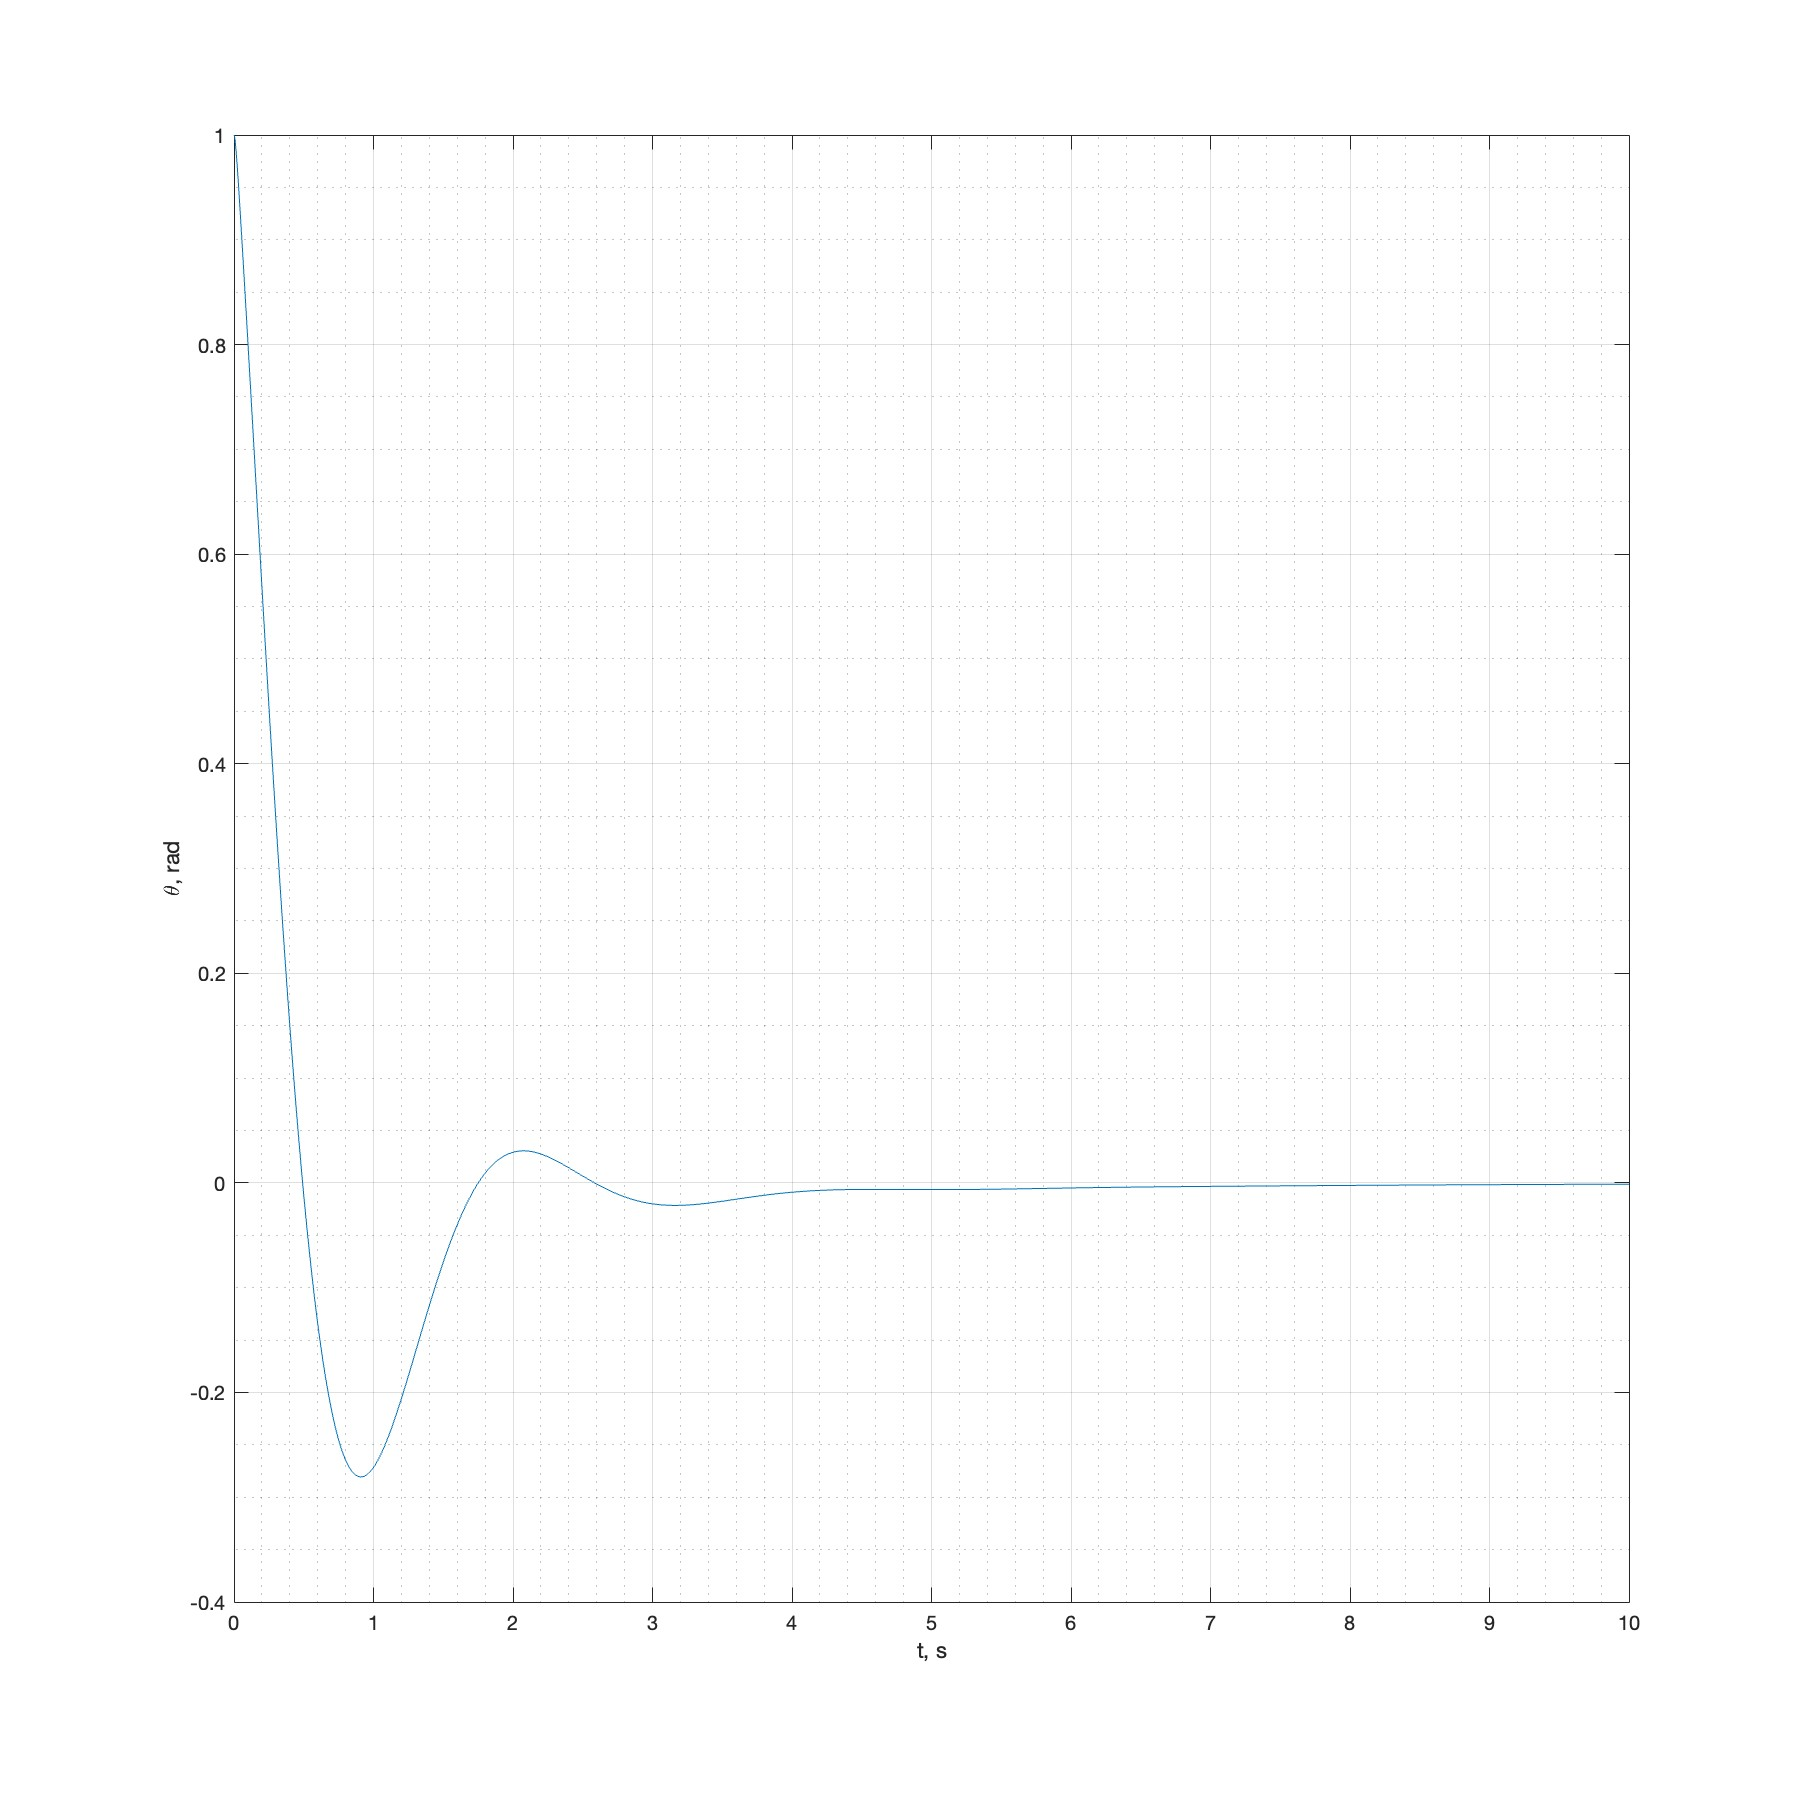
\includegraphics[width=1\linewidth]{"./graphics/tet_20_10_10.jpg"}}
                    %  \includegraphics{"./Q-table.jpg"}
	           \caption{$\Theta (t)$ при $p = 20, \, i = 10, \, d = 10$}
\end{figure}
\begin{figure}[!h]
		{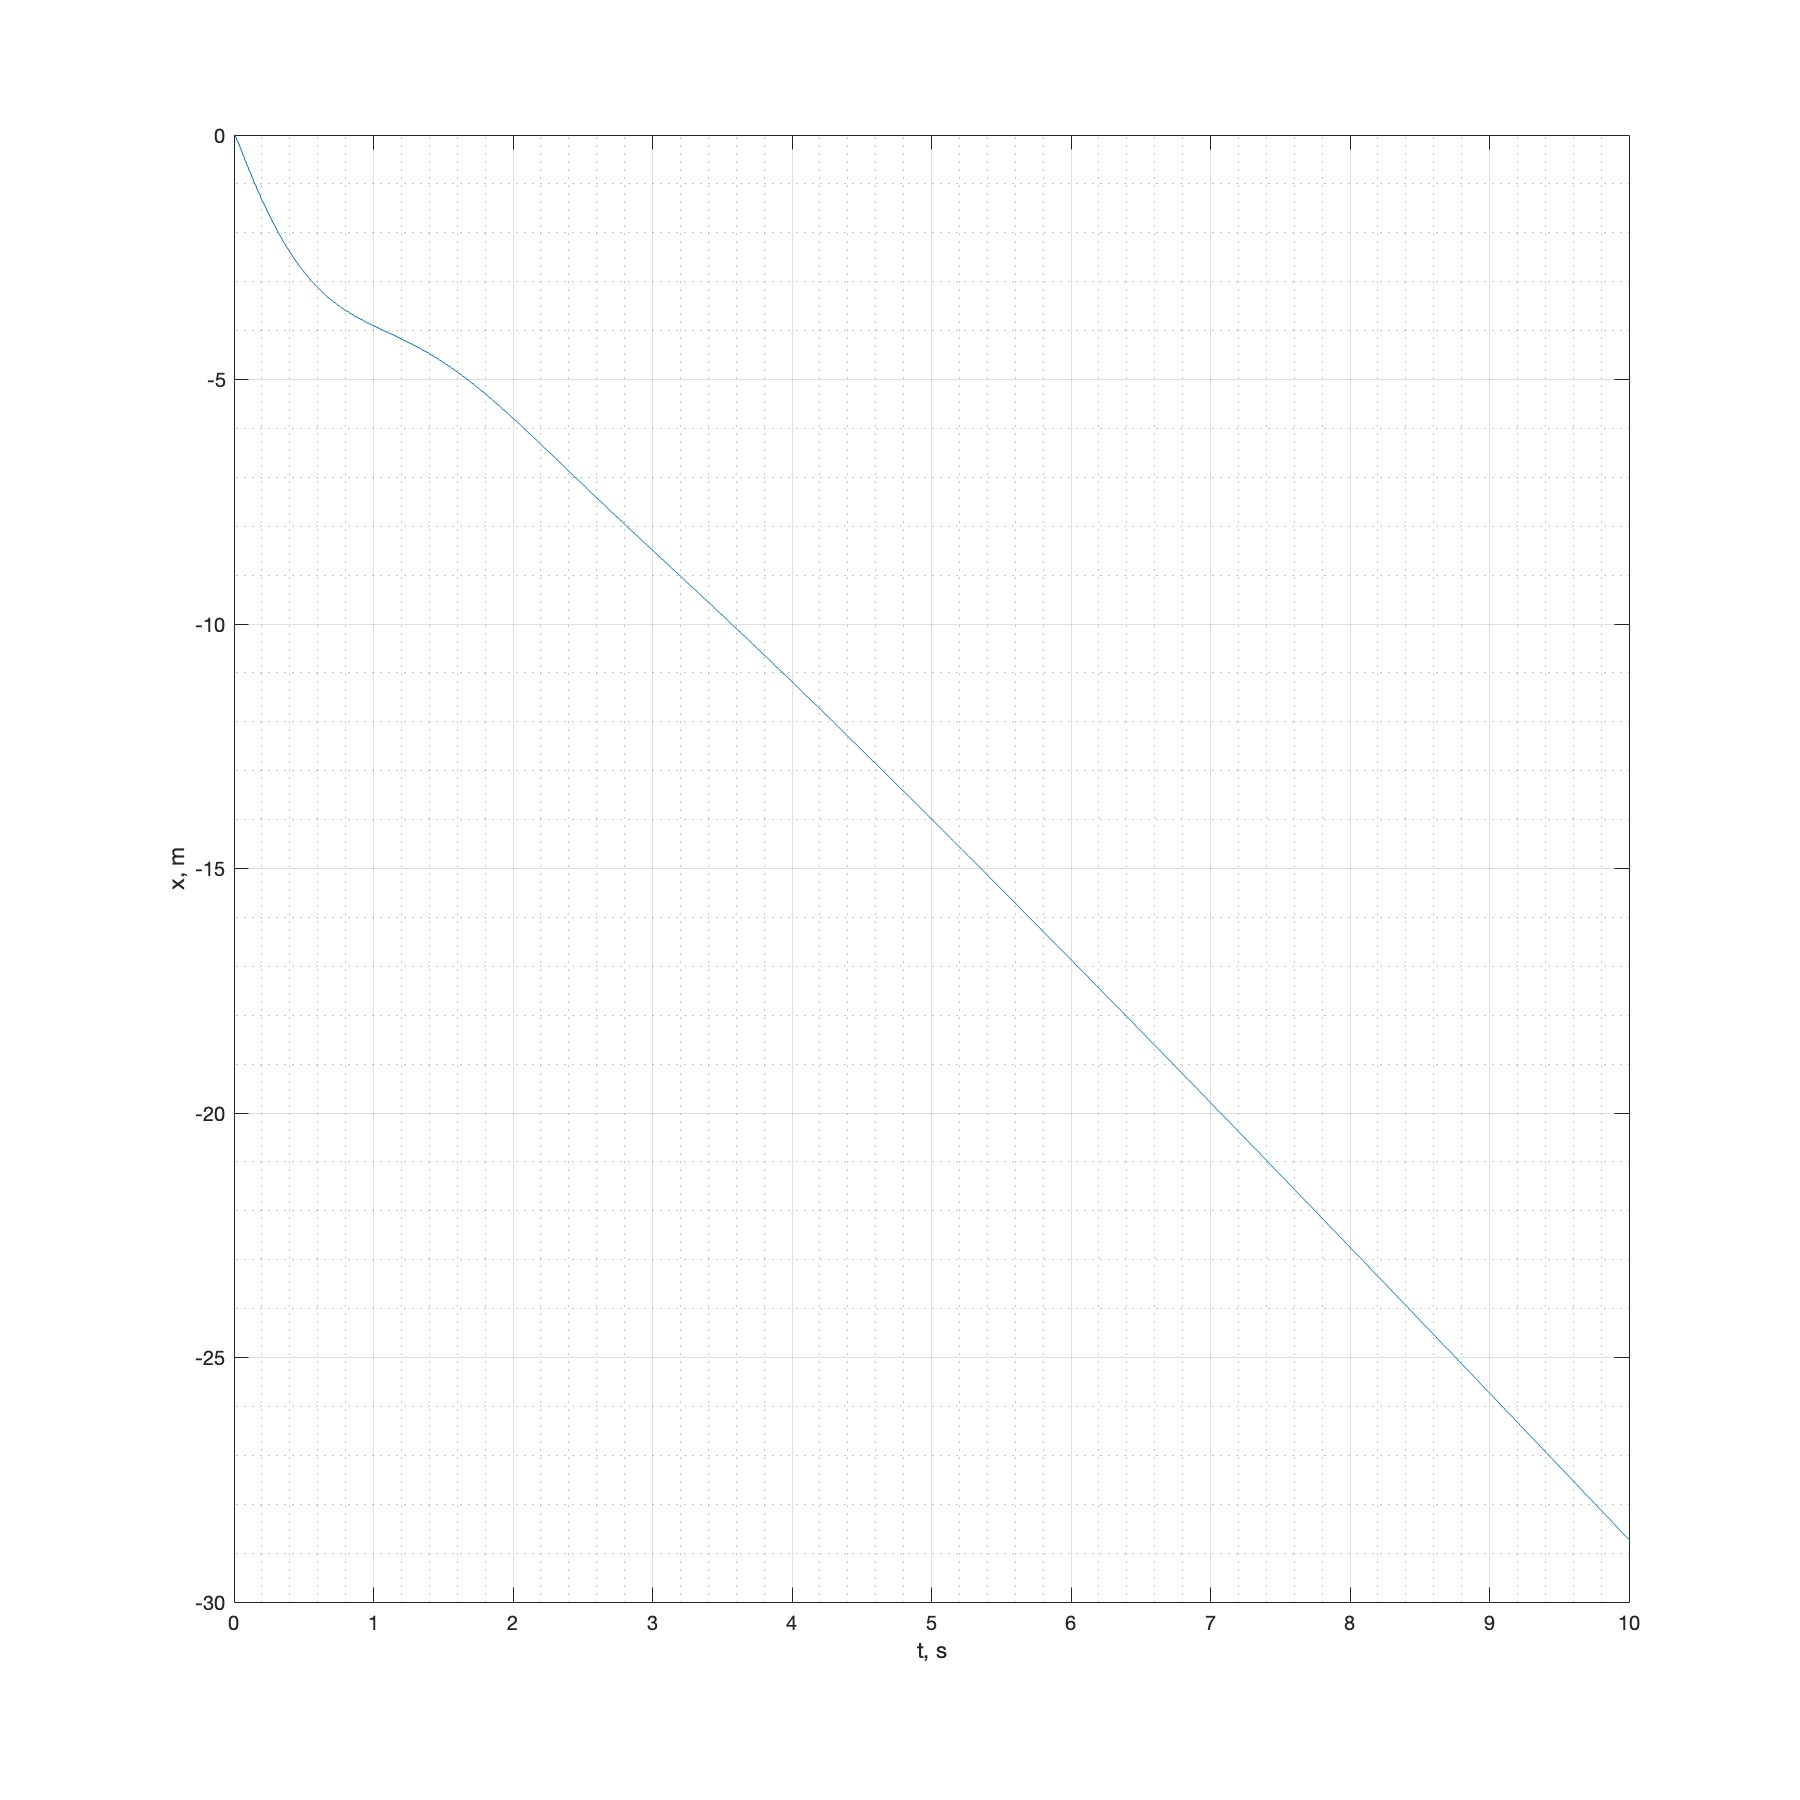
\includegraphics[width=1\linewidth]{"./graphics/x_20_10_10.jpg"}}
                    %  \includegraphics{"./Q-table.jpg"}
	           \caption{$x(t)$  при $p = 20, \, i = 10, \, d = 10$}
\end{figure}
\begin{figure}[!h]
		{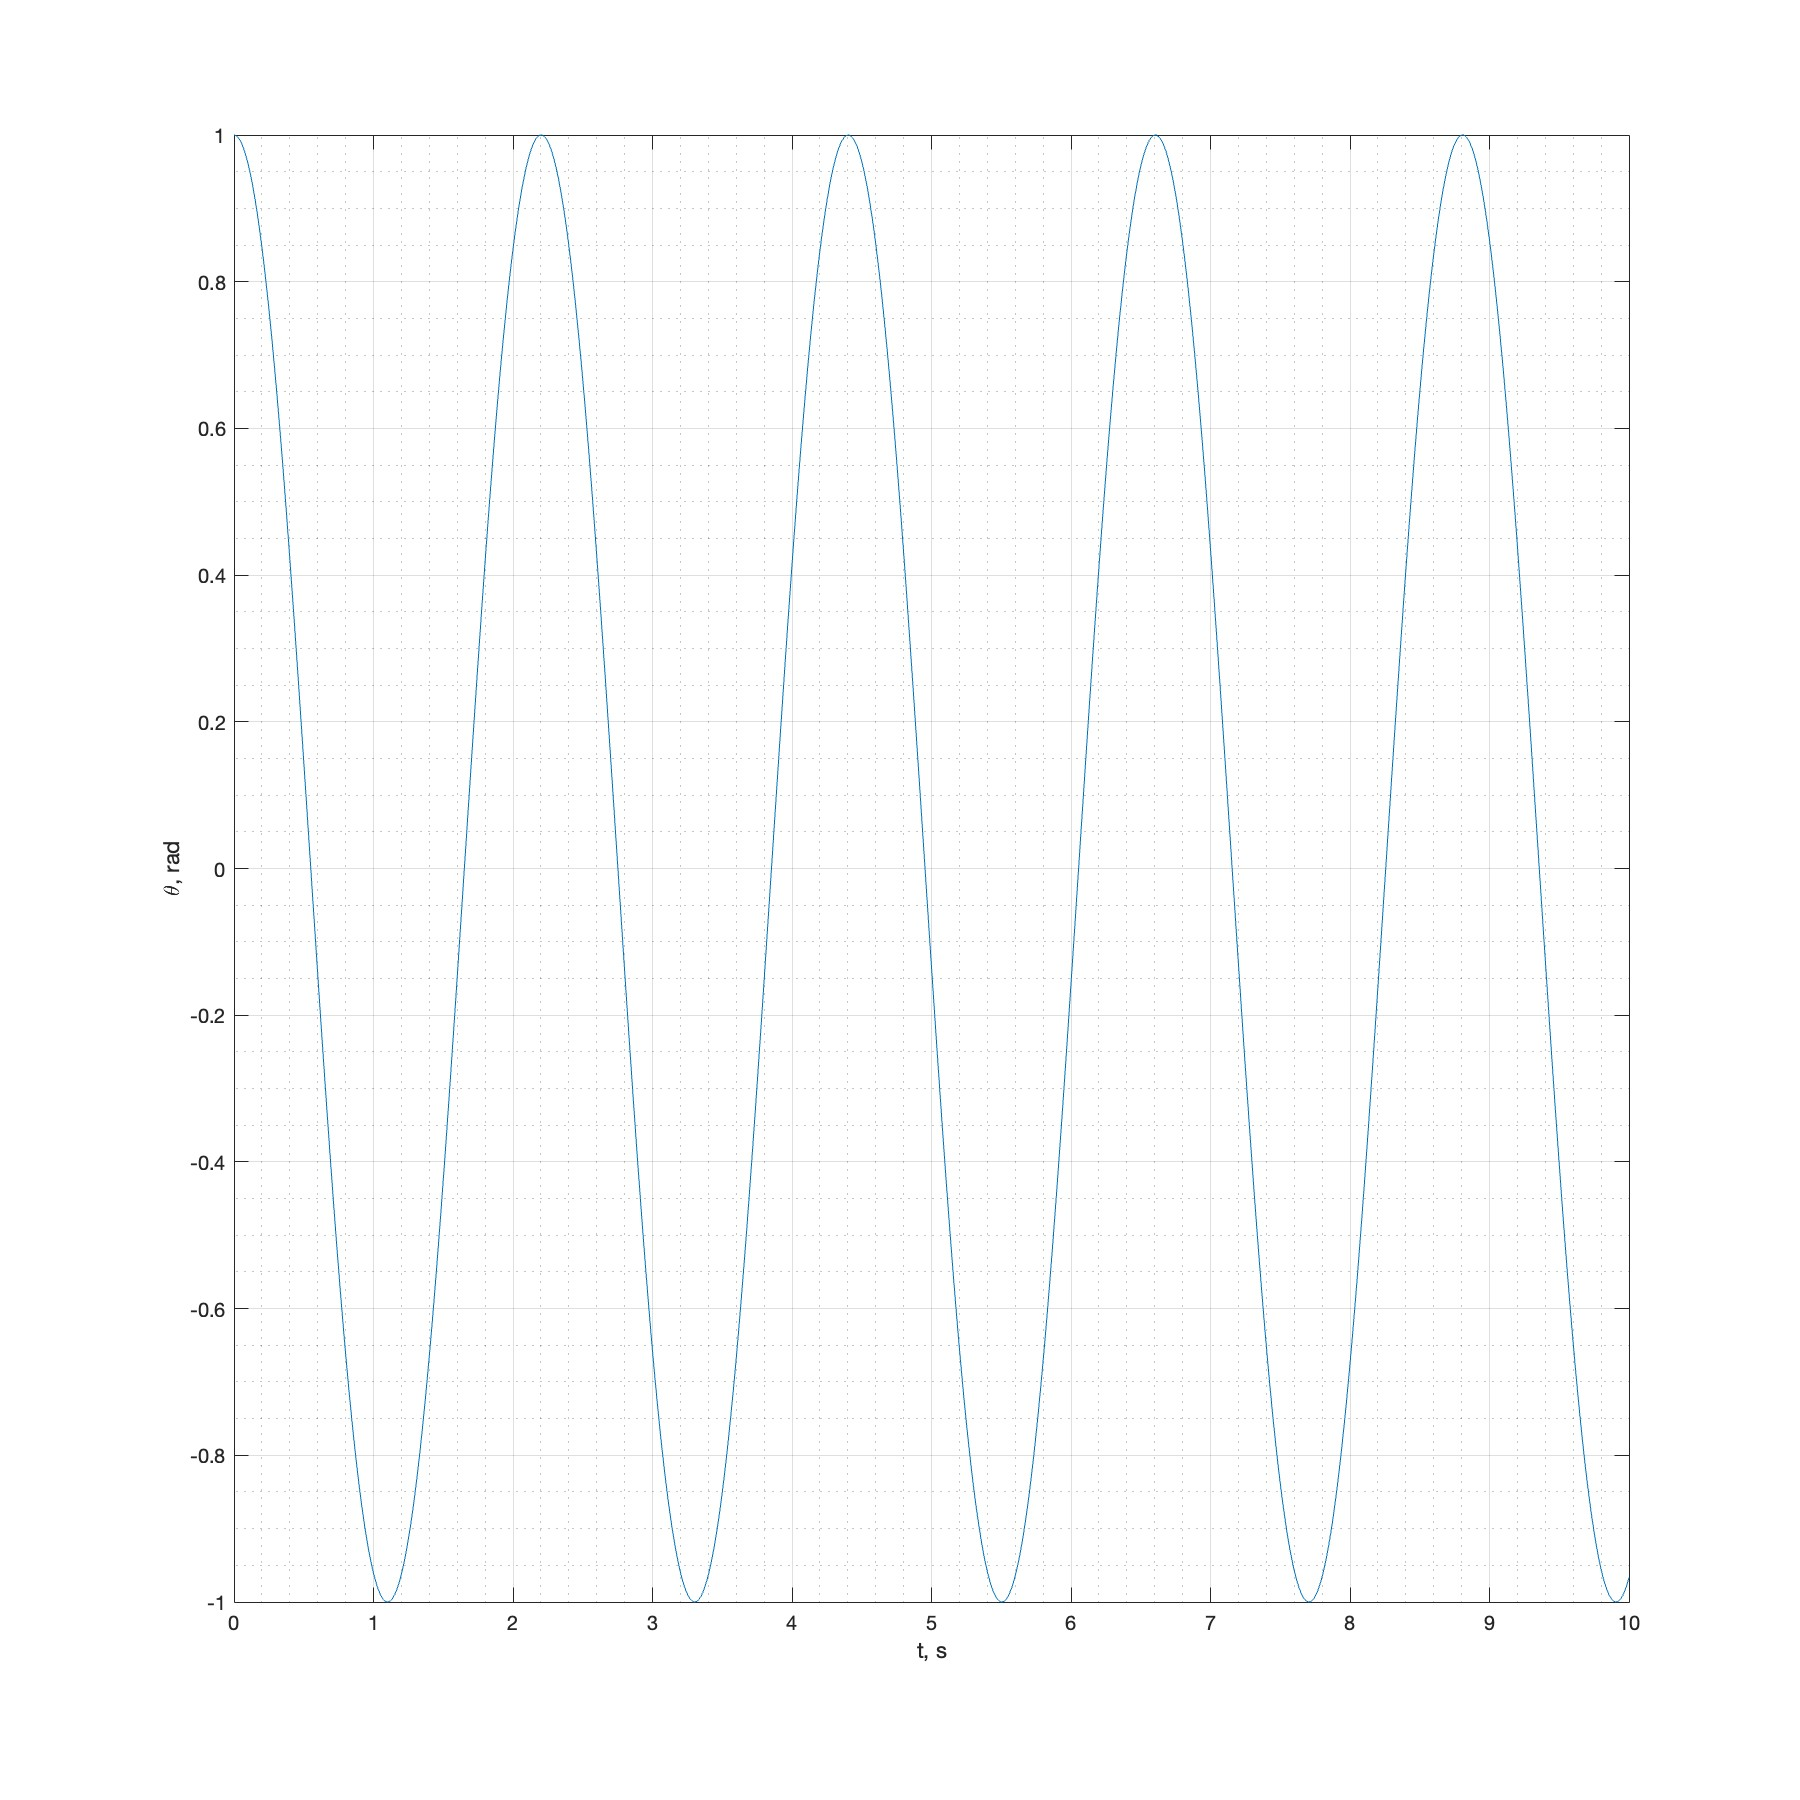
\includegraphics[width=1\linewidth]{"./graphics/tet_20_0_0.jpg"}}
                    %  \includegraphics{"./Q-table.jpg"}
	           \caption{$\Theta (t)$ при $p = 20, \, i = 0, \, d = 0$}
\end{figure}
\begin{figure}[!h]
		{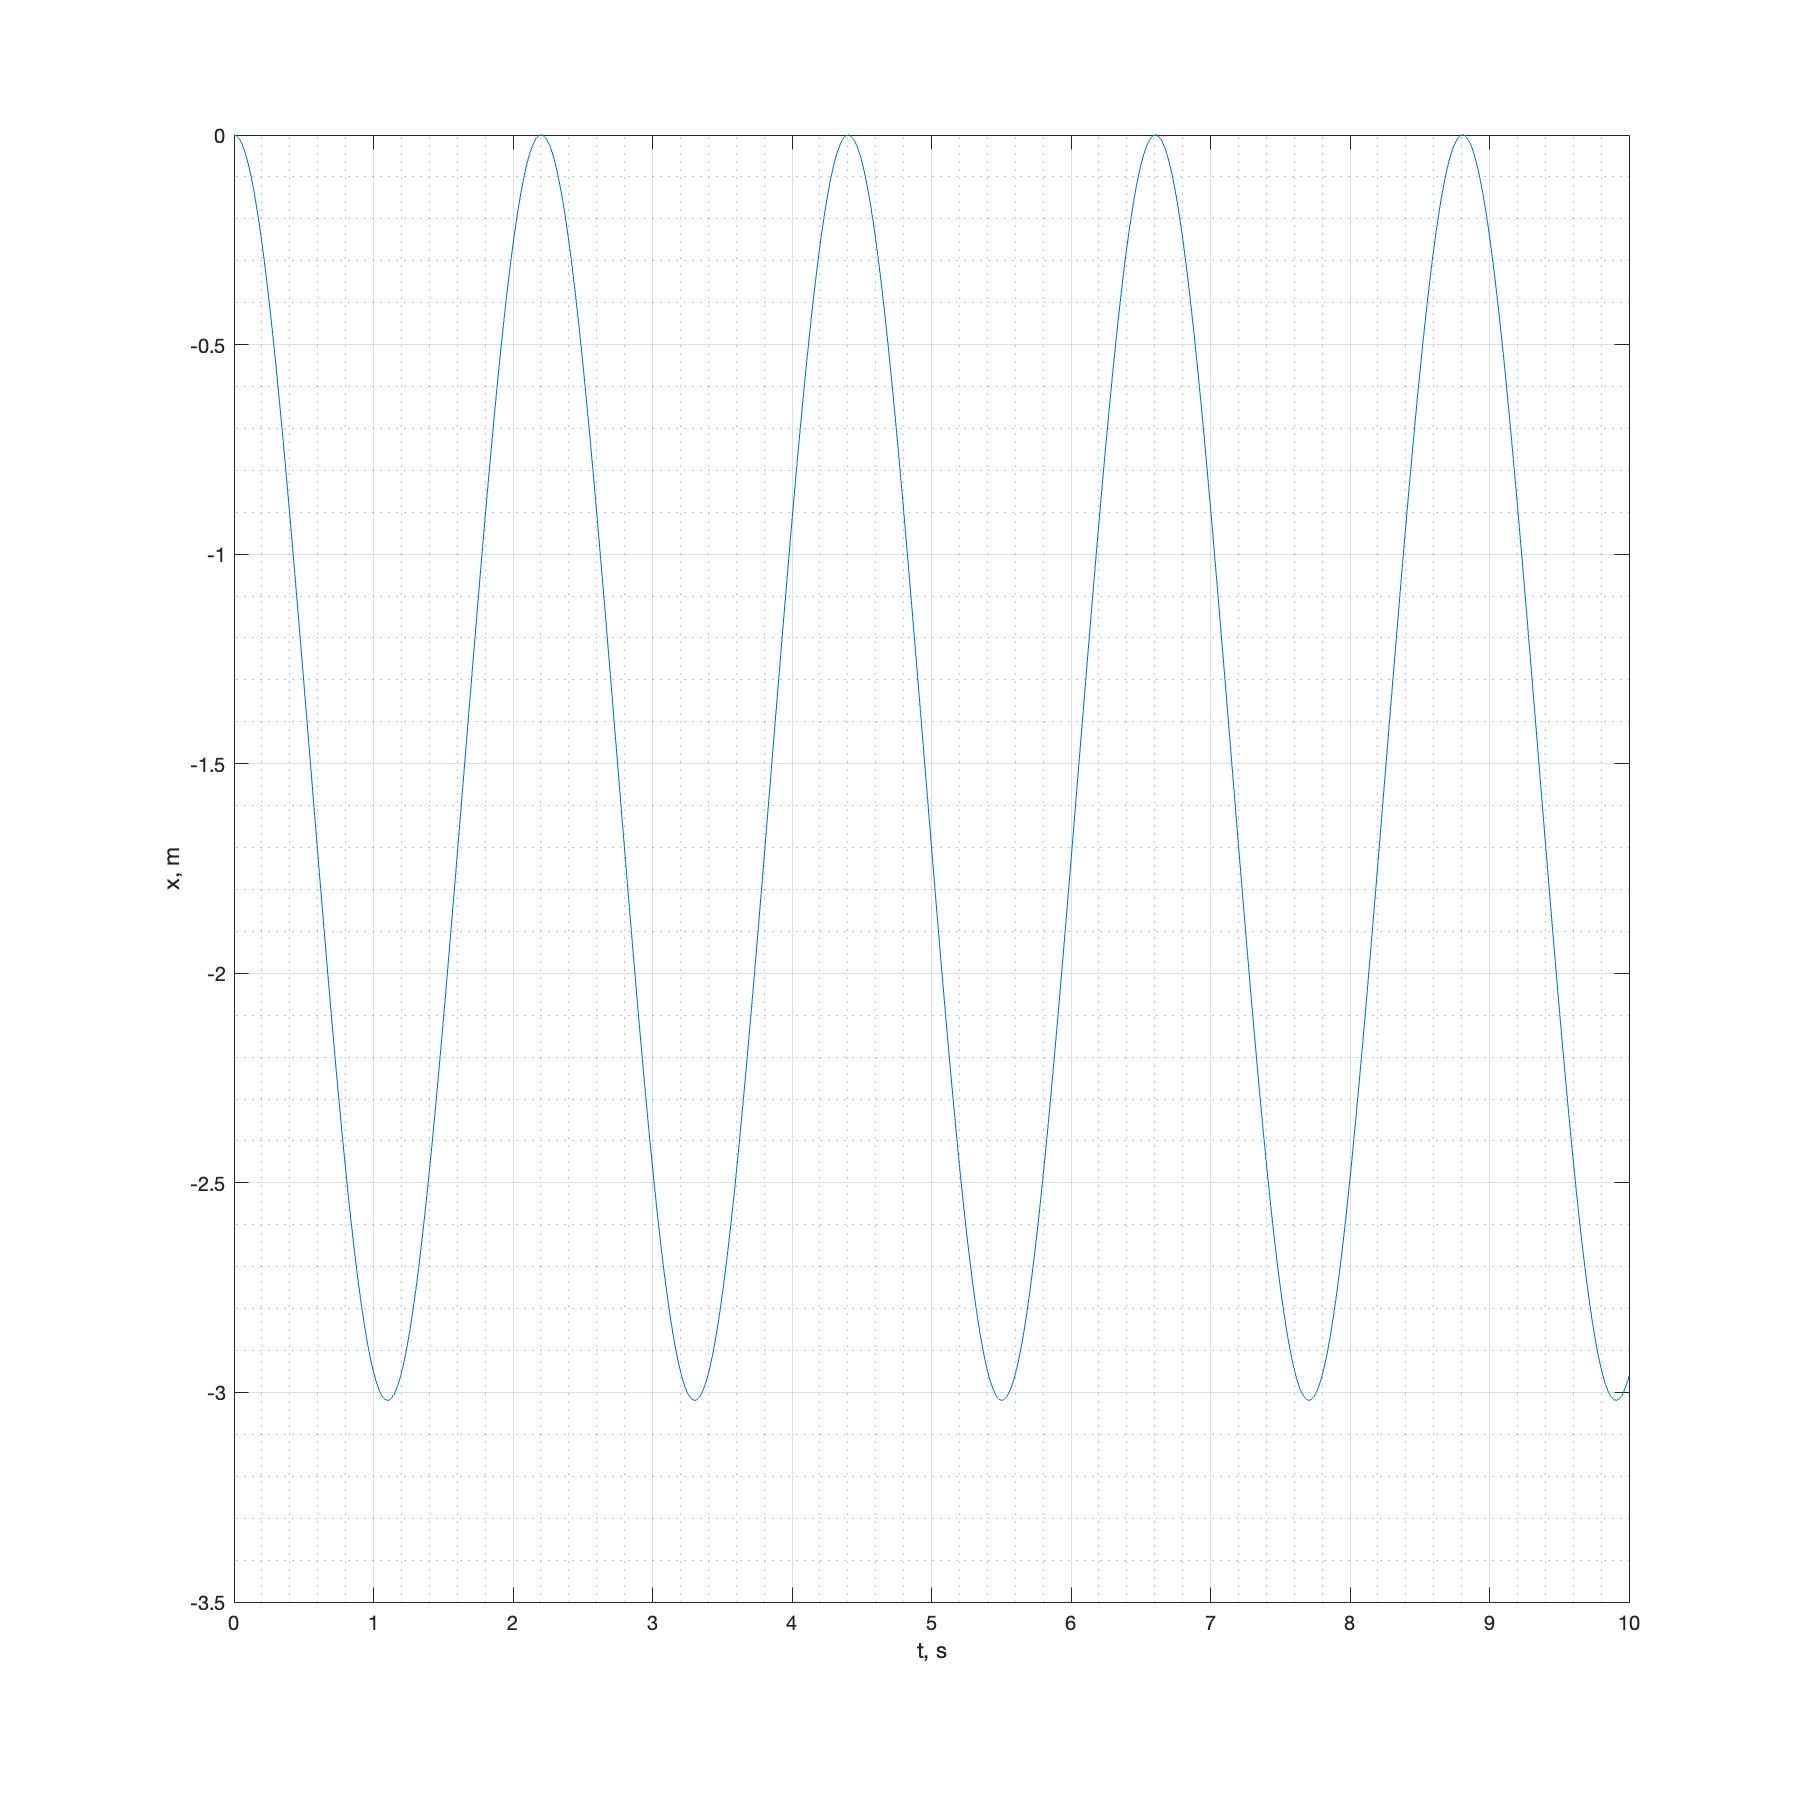
\includegraphics[width=1\linewidth]{"./graphics/x_20_0_0.jpg"}}
                    %  \includegraphics{"./Q-table.jpg"}
	           \caption{$x(t)$  при $p = 20, \, i = 0, \, d = 0$}
\end{figure}
\begin{figure}[!h]
		{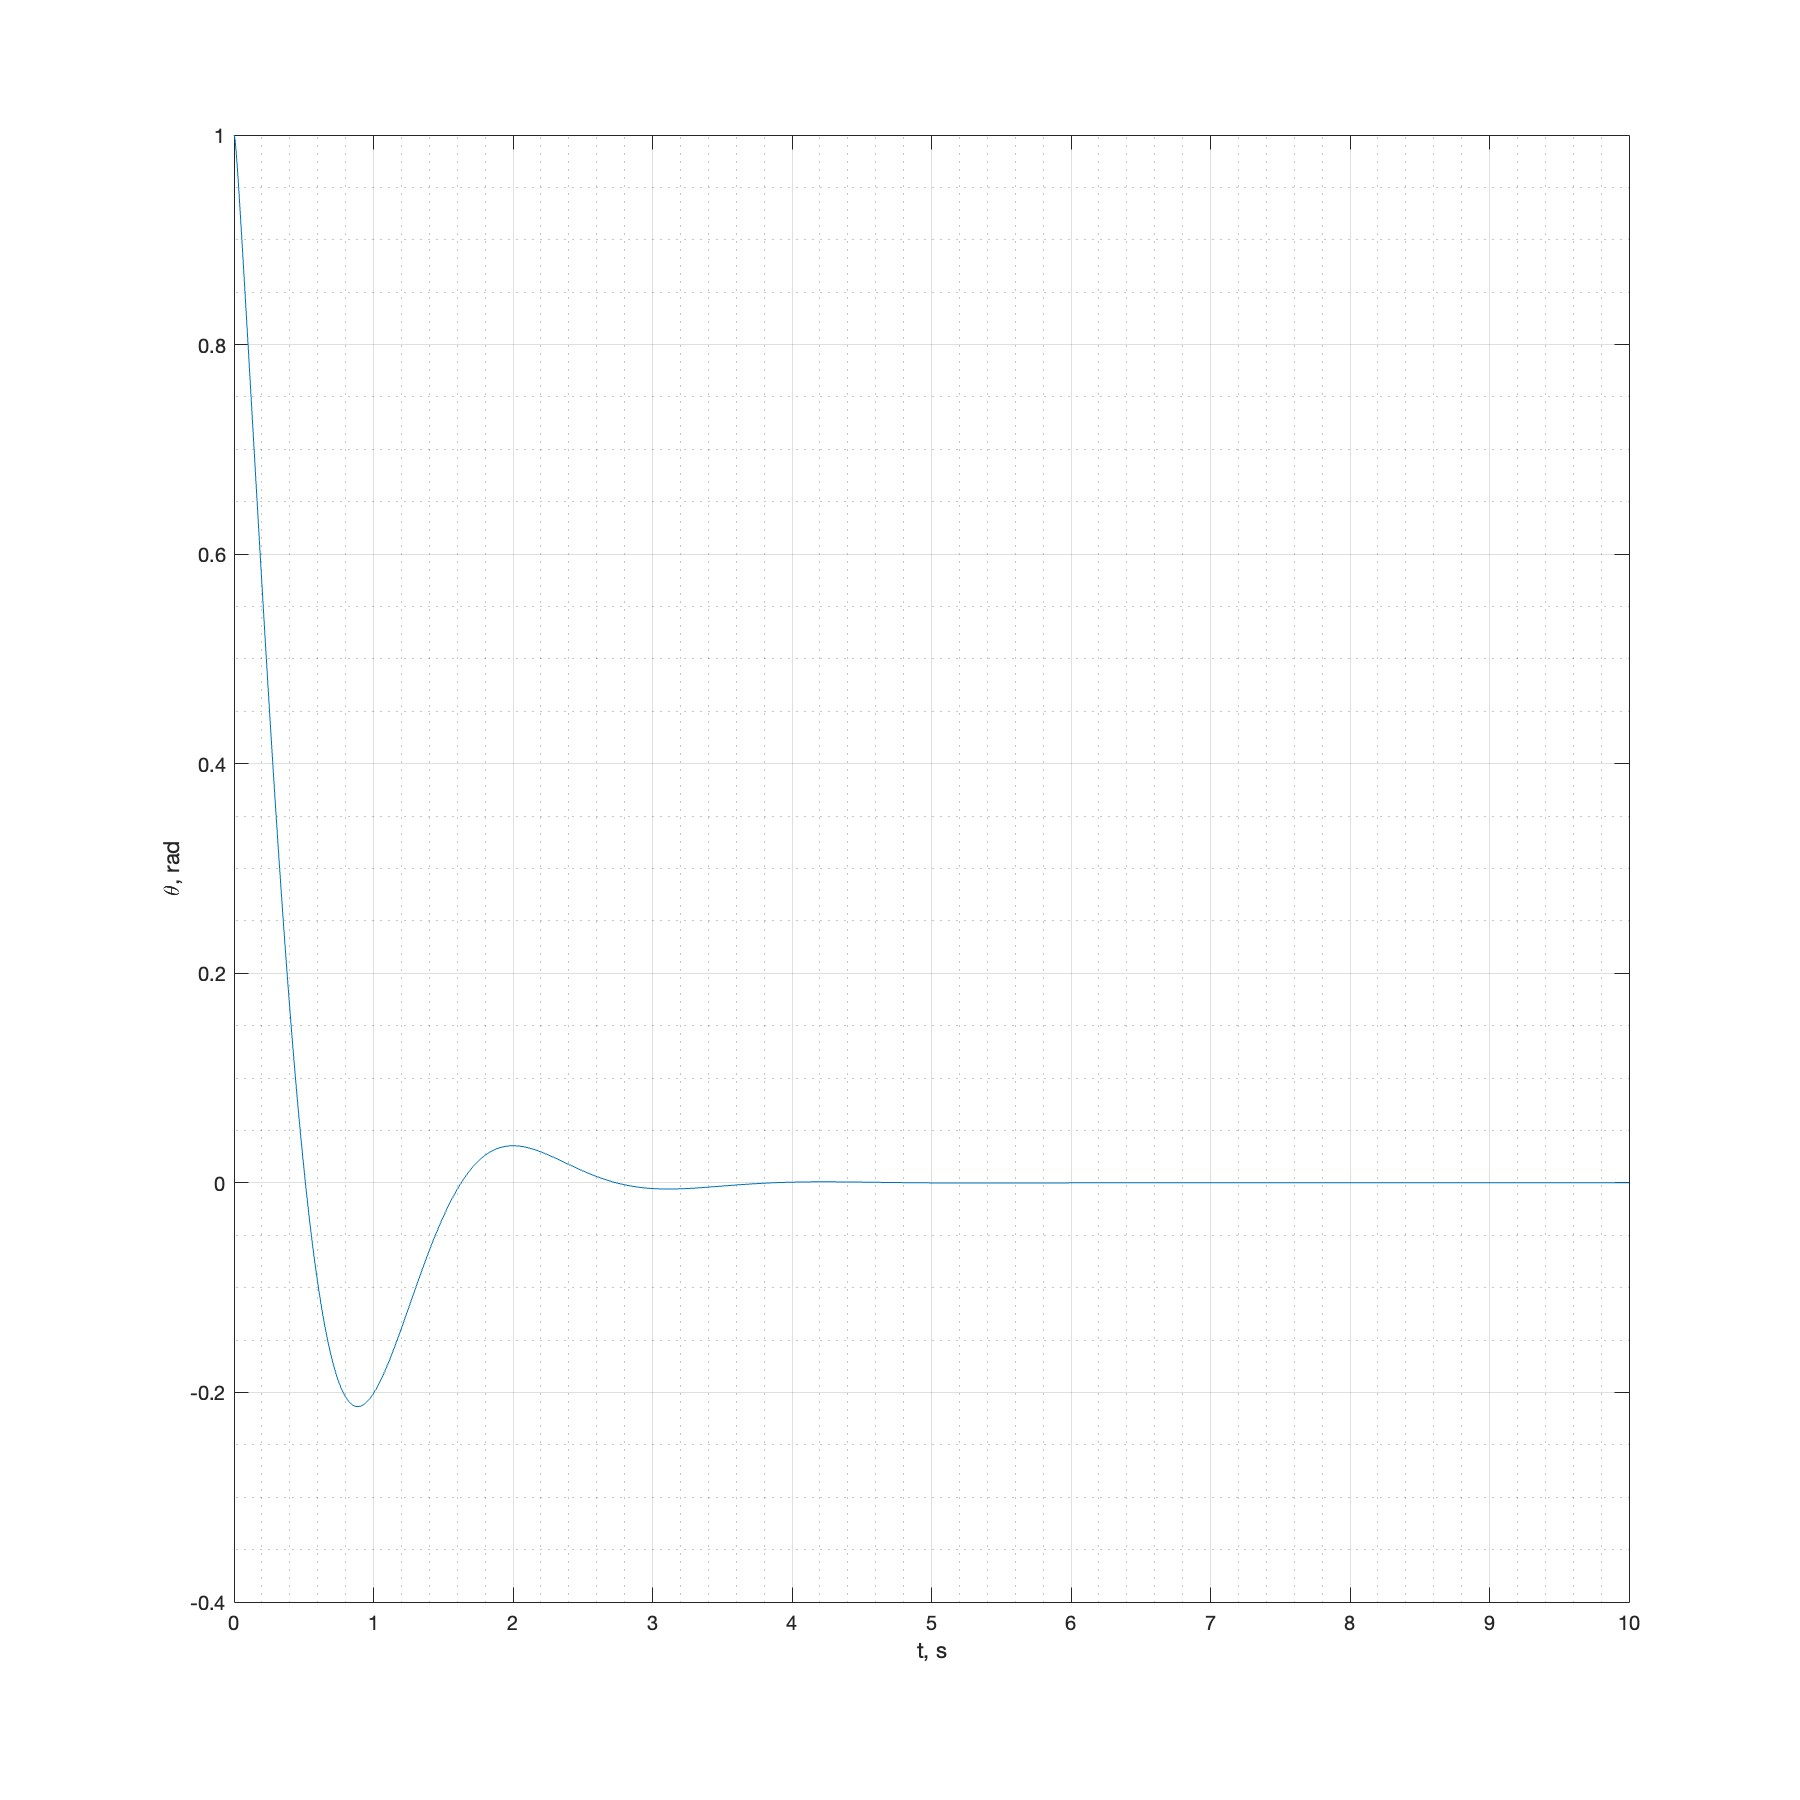
\includegraphics[width=1\linewidth]{"./graphics/x_20_10_0.jpg"}}
                    %  \includegraphics{"./Q-table.jpg"}
	           \caption{$\Theta (t)$ при $p = 20, \, i = 10, \, d = 0$}
\end{figure}
\begin{figure}[!h]
		{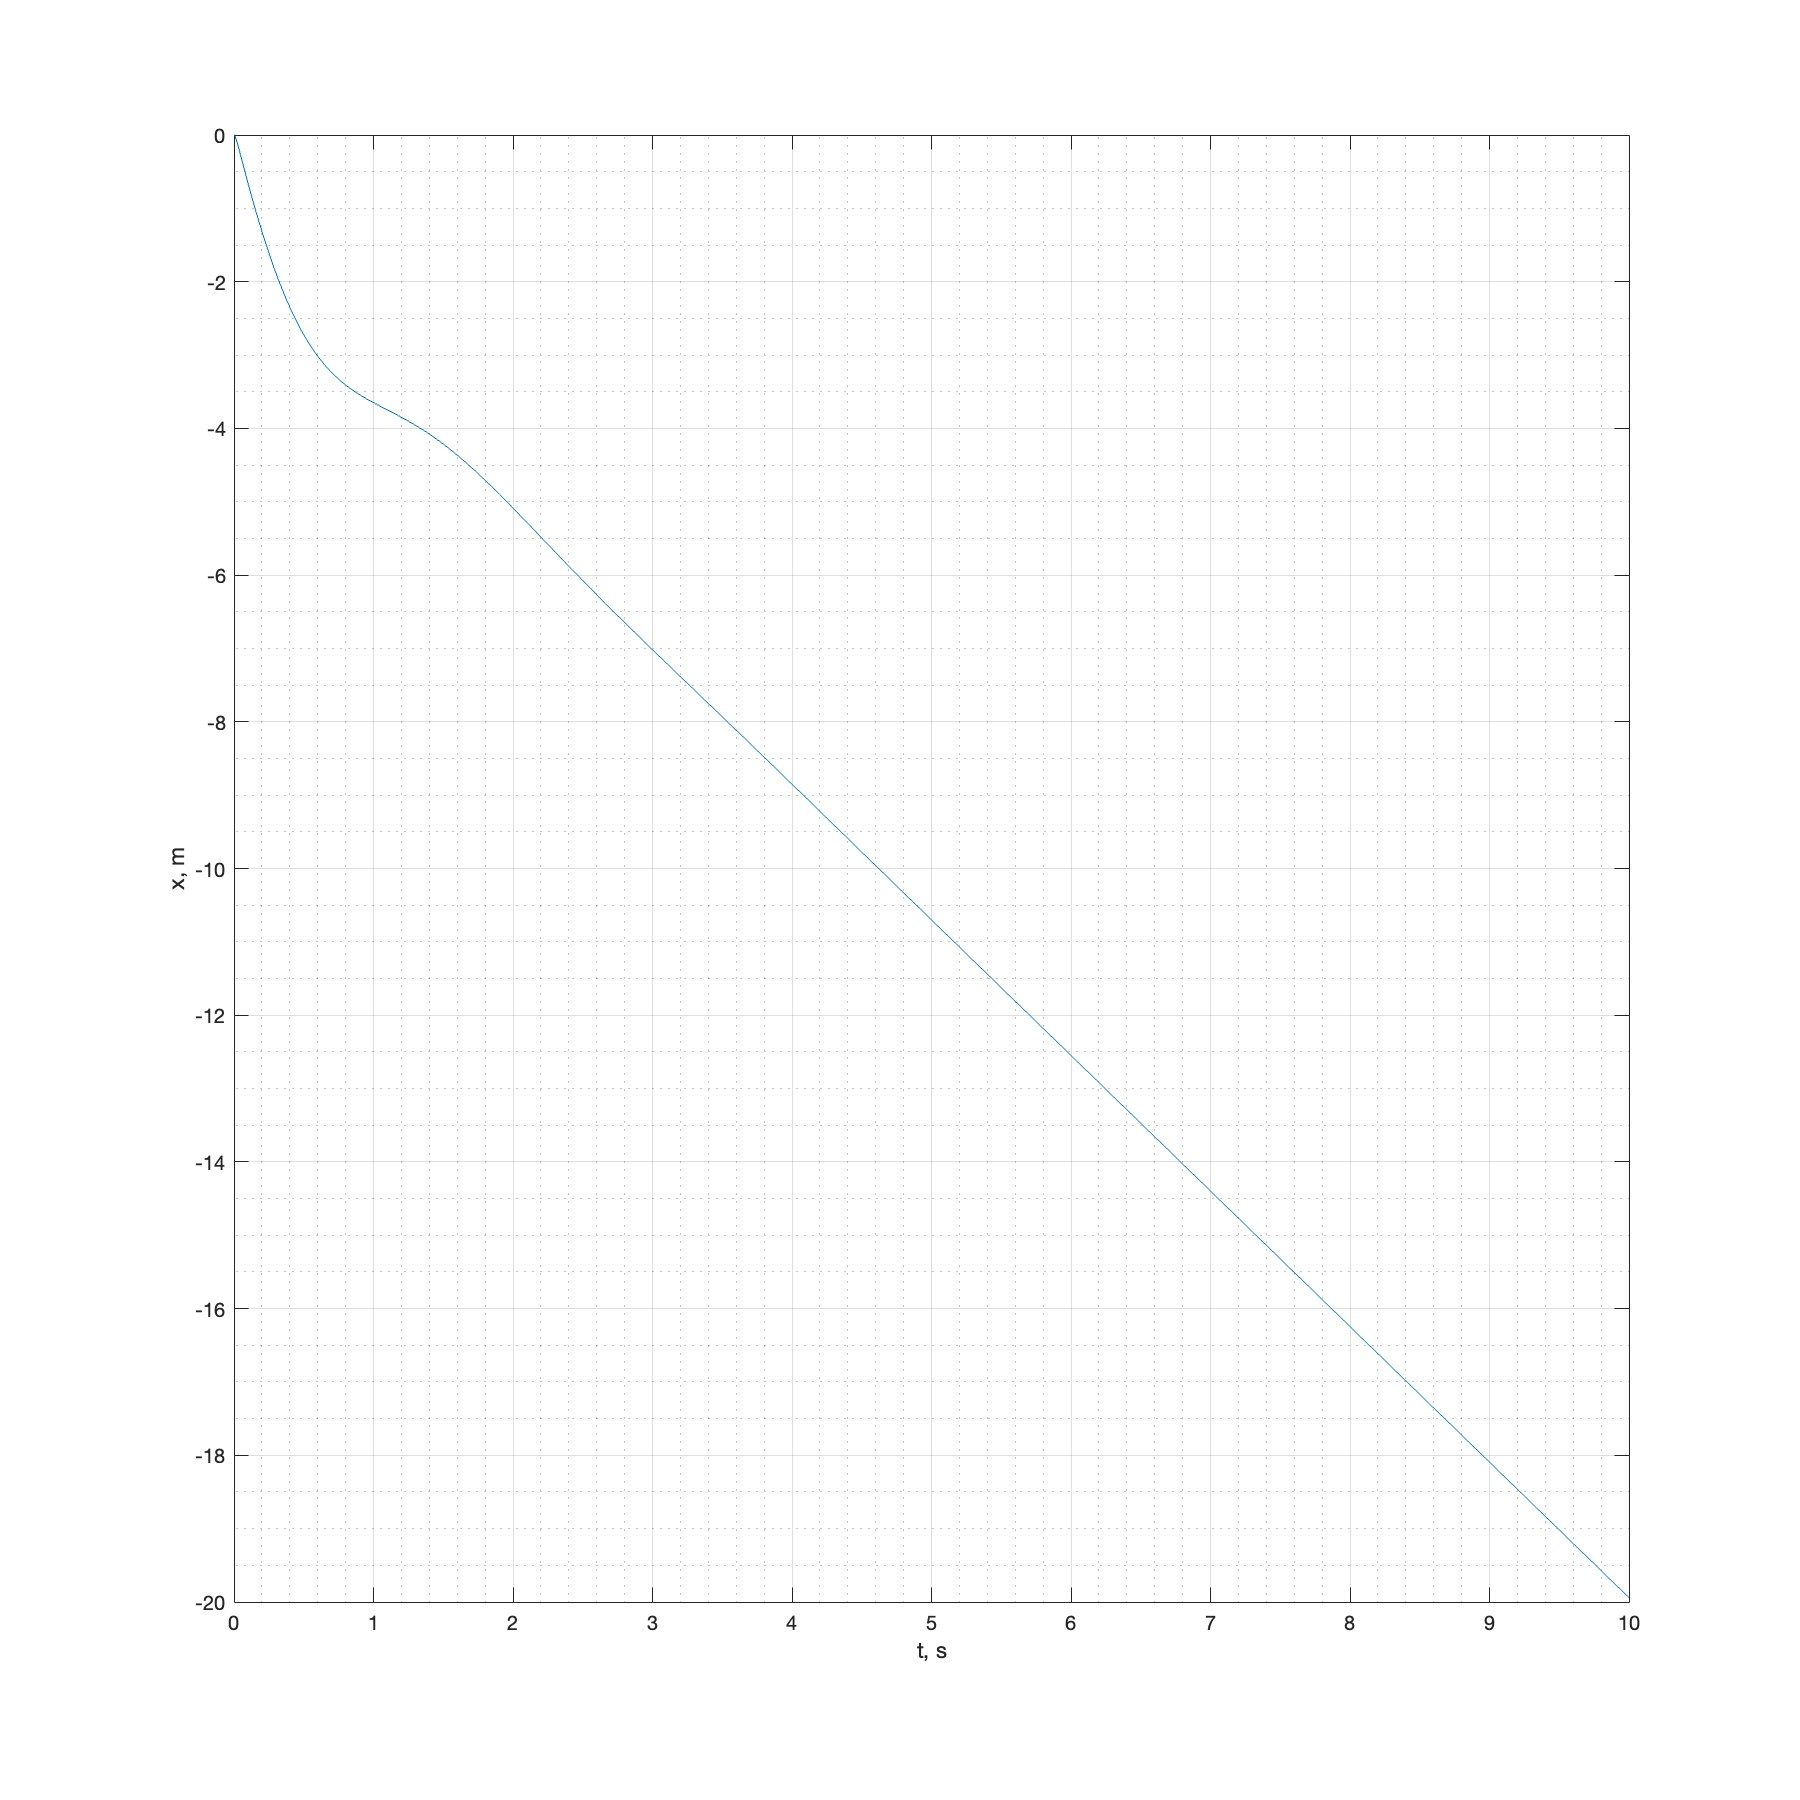
\includegraphics[width=1\linewidth]{"./graphics/tet_20_10_0.jpg"}}
                    %  \includegraphics{"./Q-table.jpg"}
	           \caption{$x(t)$  при $p = 20, \, i = 10, \, d = 0$}
\end{figure}
\begin{figure}[!h]
		{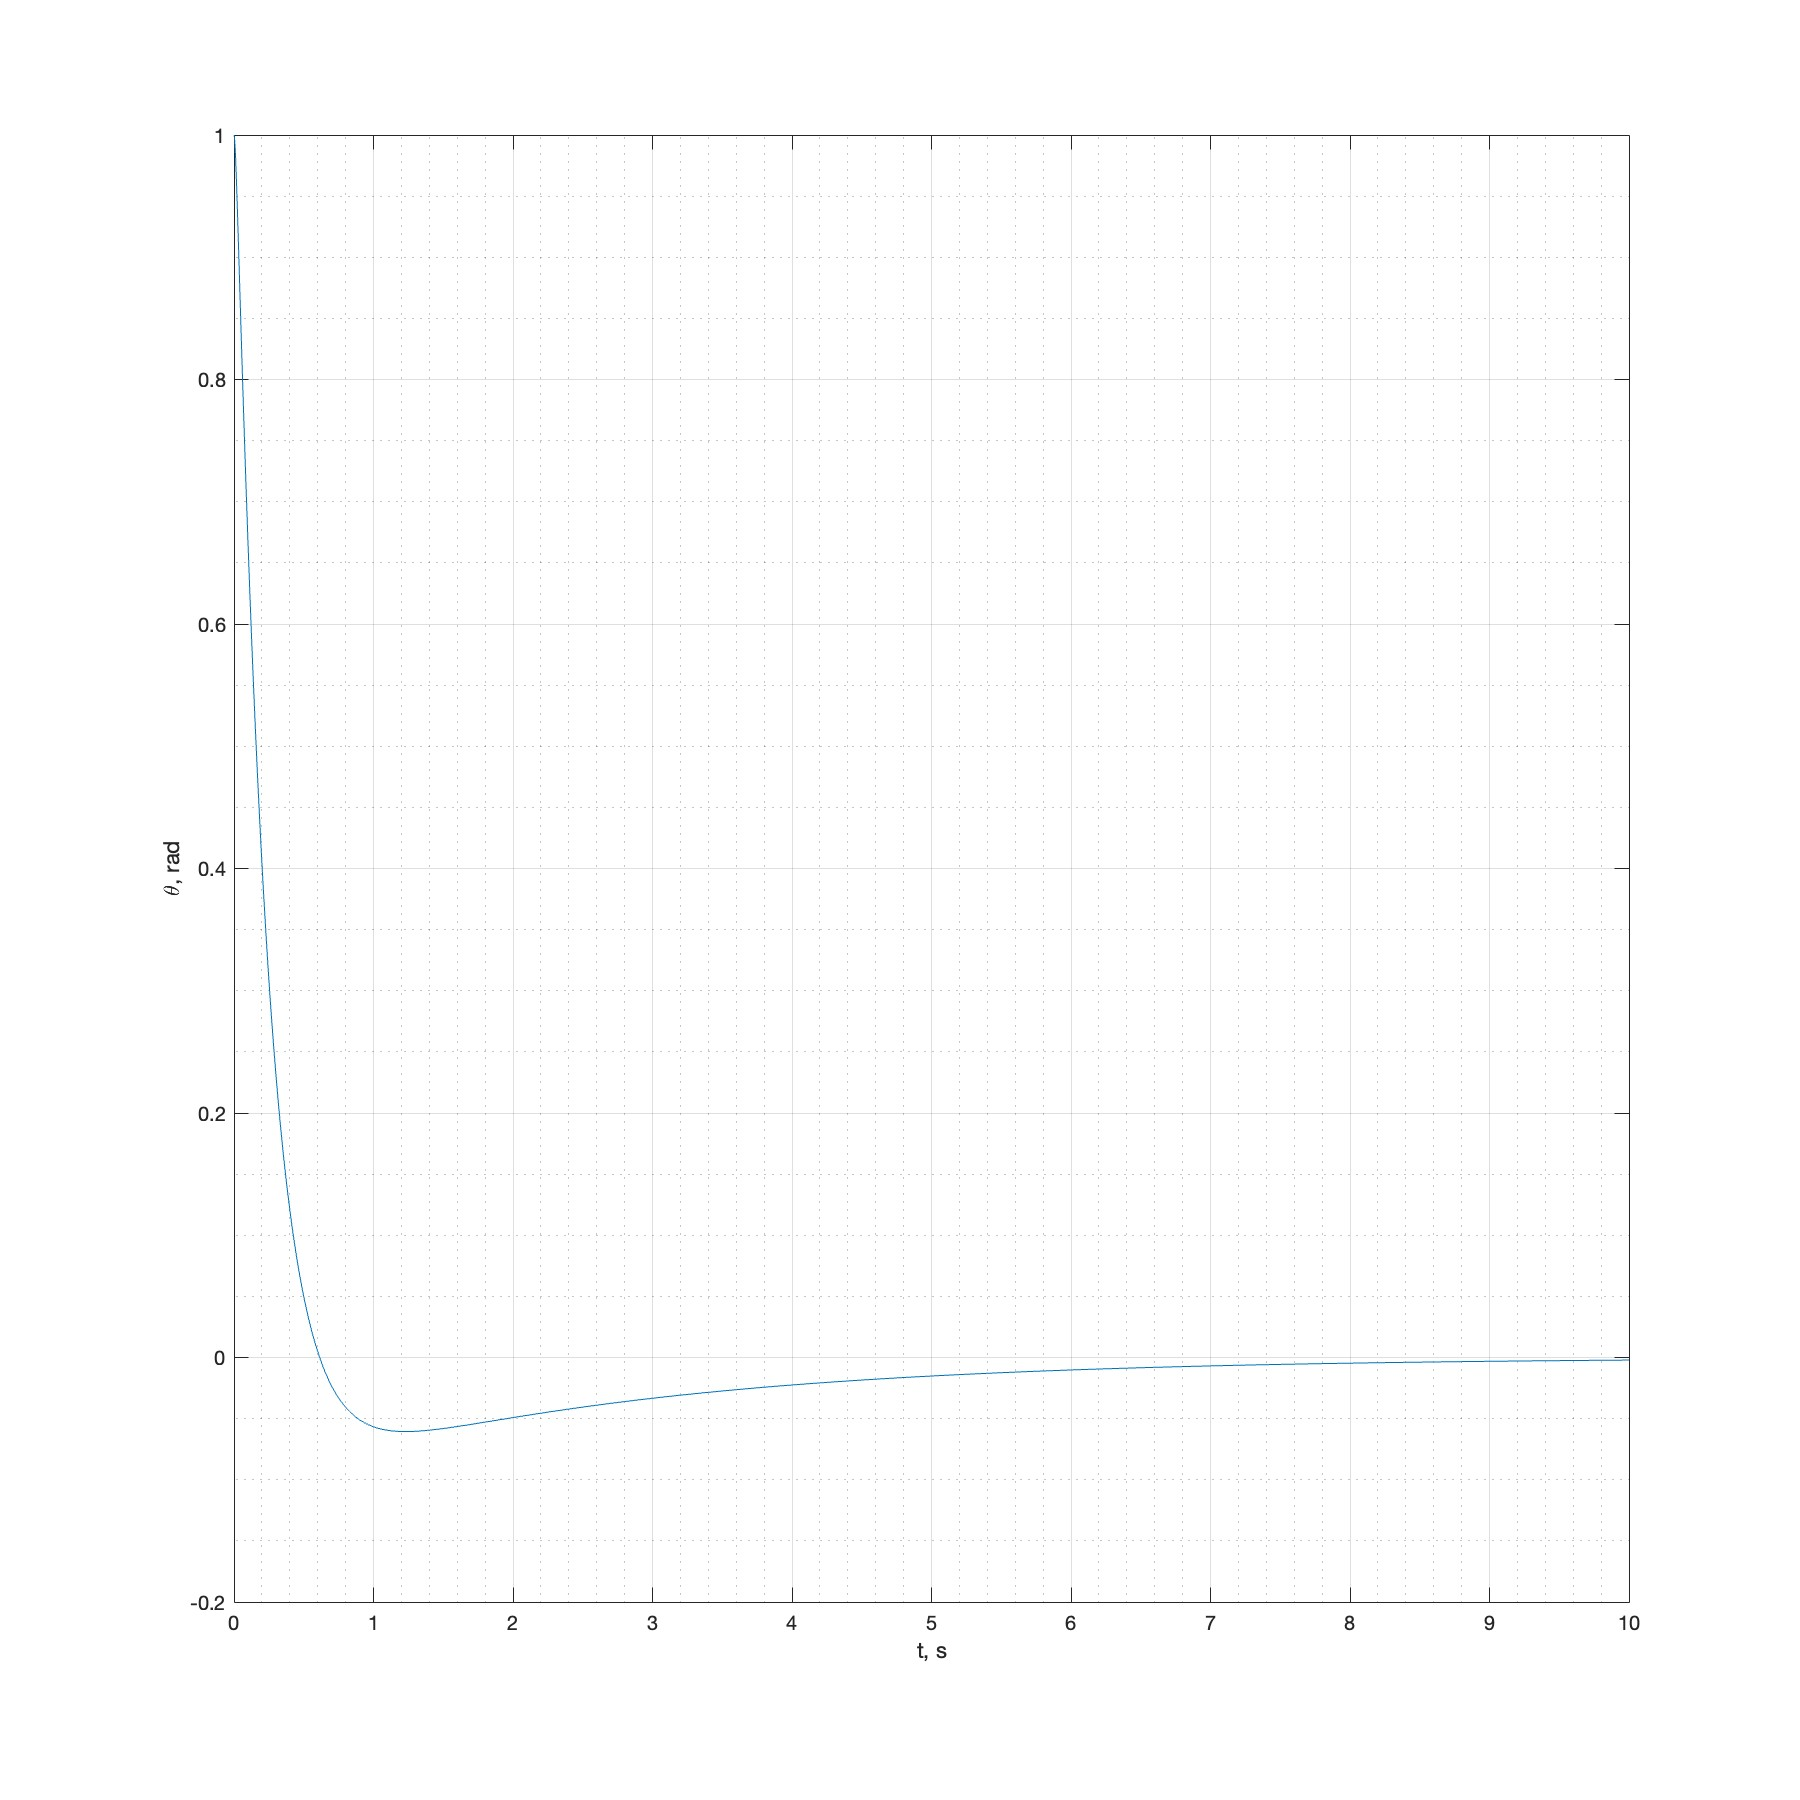
\includegraphics[width=1\linewidth]{"./graphics/tet_20_10_20.jpg"}}
                    %  \includegraphics{"./Q-table.jpg"}
	           \caption{$\Theta (t)$ при $p = 20, \, i = 10, \, d = 20$}
\end{figure}
\begin{figure}[!h]
		{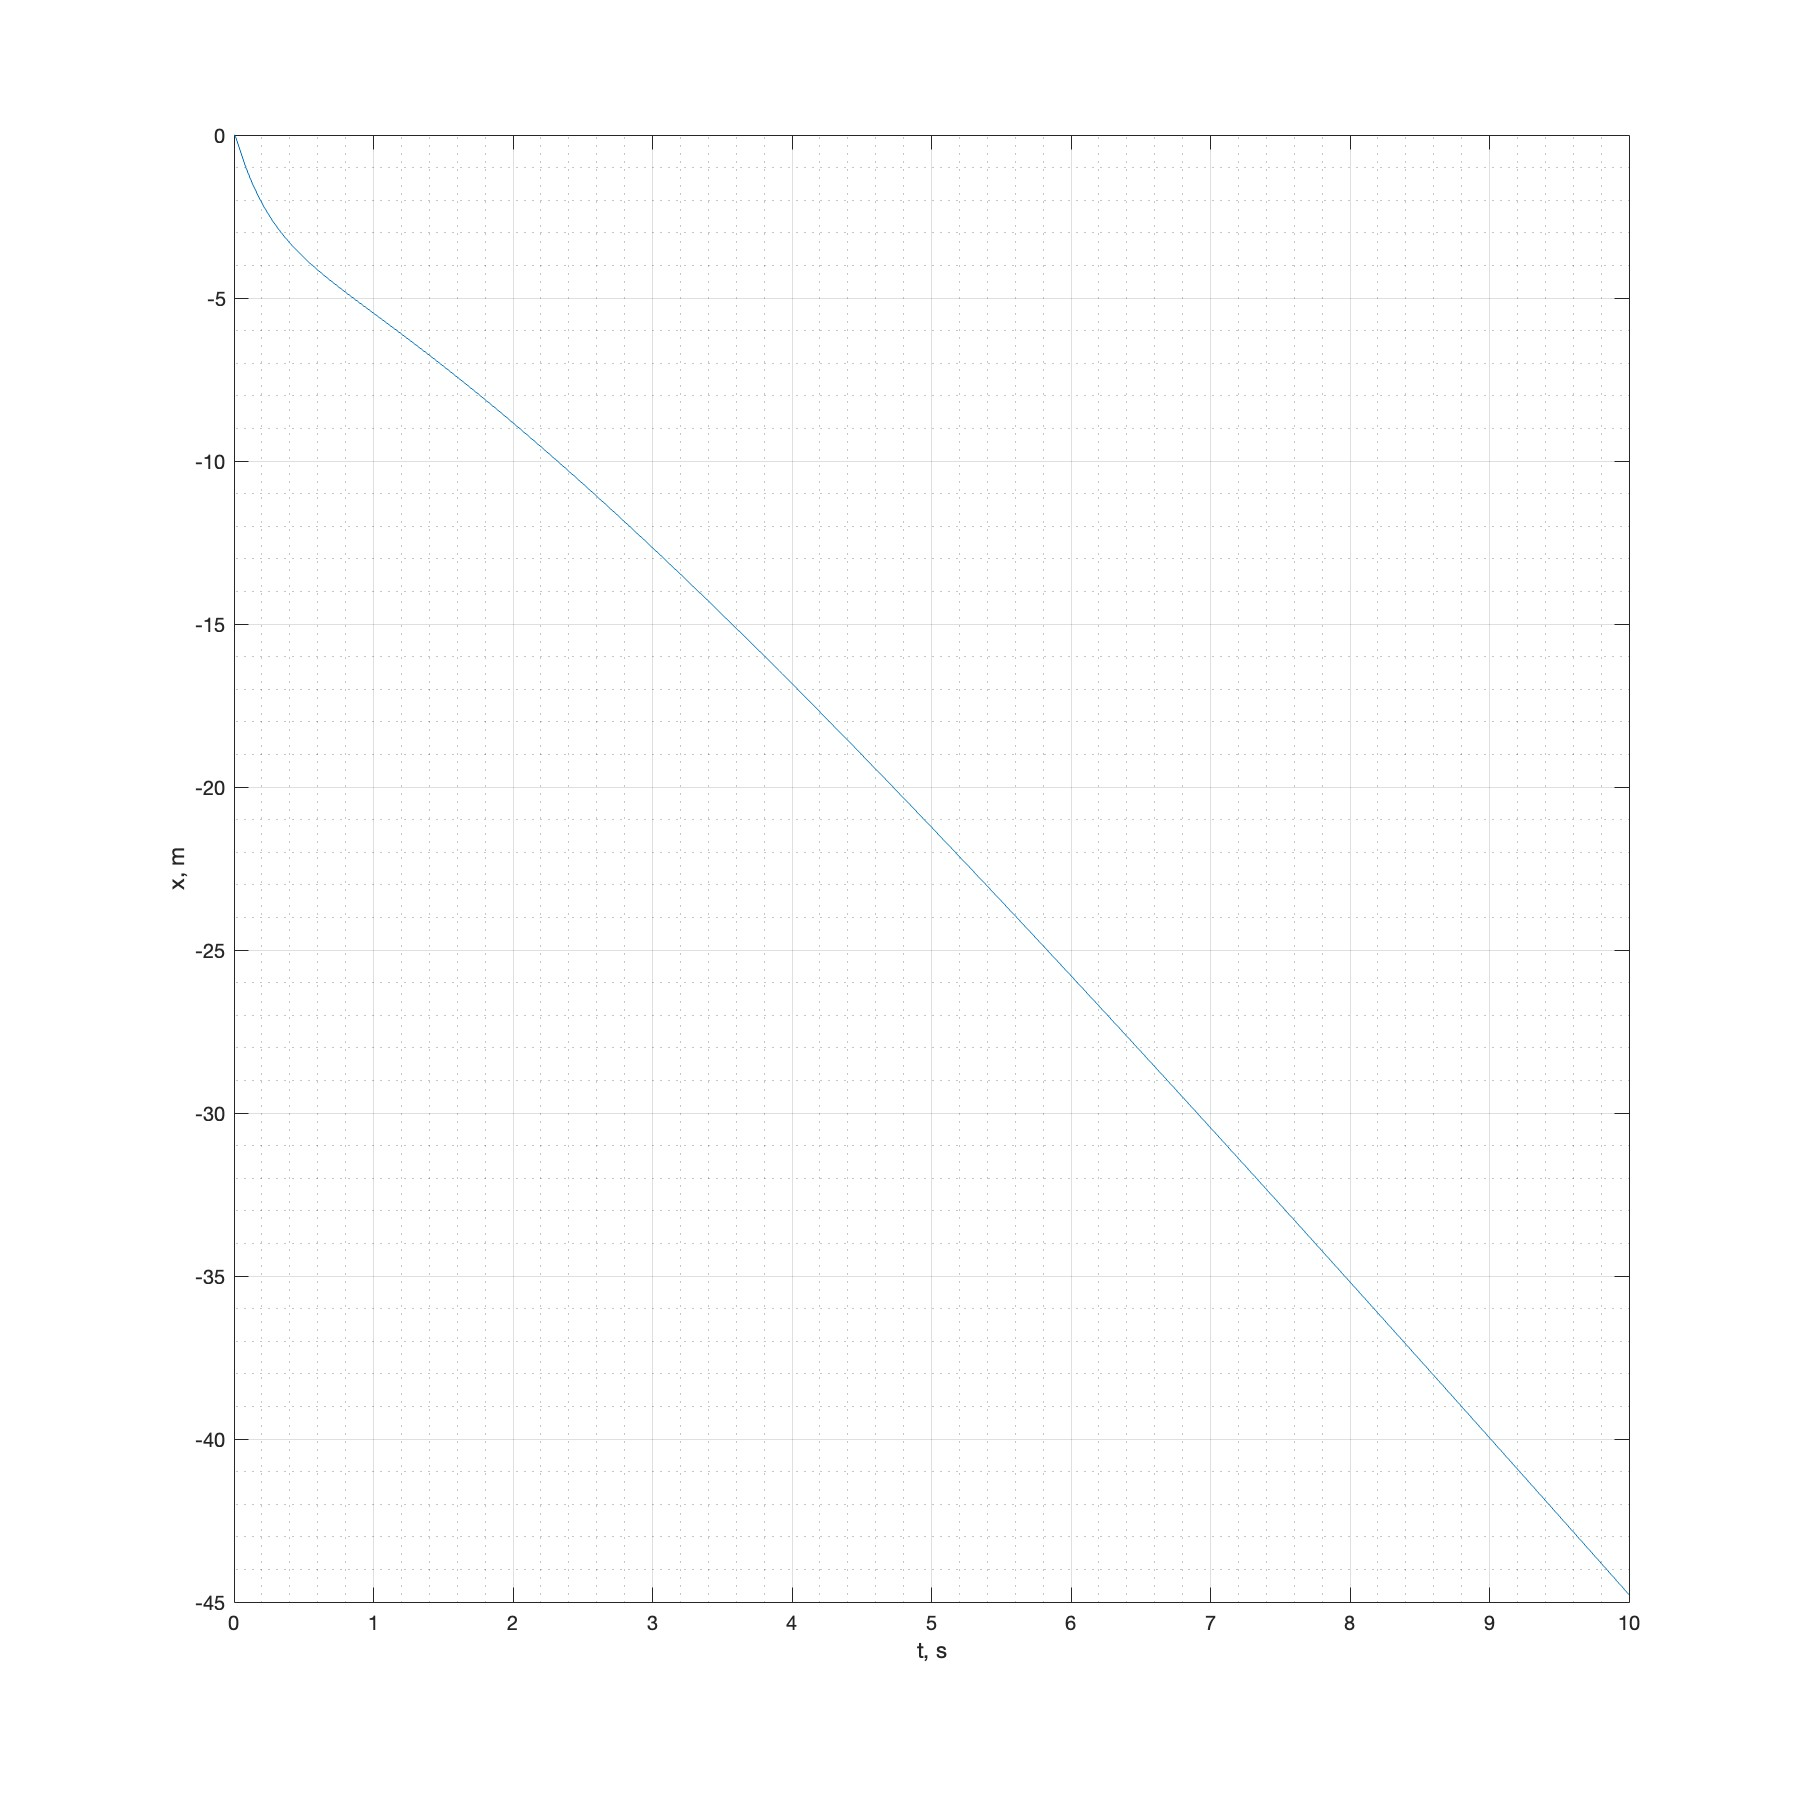
\includegraphics[width=1\linewidth]{"./graphics/x_20_10_20.jpg"}}
                    %  \includegraphics{"./Q-table.jpg"}
	           \caption{$x(t)$  при $p = 20, \, i = 10, \, d = 20$}
\end{figure}




\end{document}













